\documentclass[titlepage]{article}

\usepackage{titling}
\usepackage[margin=1in]{geometry}
\usepackage[strings]{underscore}
\usepackage{etoolbox}
\usepackage{graphicx}
\usepackage{xcolor}
\usepackage{listings}

\definecolor{mGreen}{rgb}{0,0.6,0}
\definecolor{mGray}{rgb}{0.5,0.5,0.5}
\definecolor{mPurple}{rgb}{0.58,0,0.82}
\definecolor{backgroundColour}{rgb}{0.95,0.95,0.92}

\lstdefinestyle{CStyle}{
    backgroundcolor=\color{backgroundColour},   
    commentstyle=\color{mGreen},
    keywordstyle=\color{magenta},
    numberstyle=\tiny\color{mGray},
    stringstyle=\color{mPurple},
    basicstyle=\footnotesize,
    breakatwhitespace=false,         
    breaklines=true,                 
    captionpos=b,                    
    keepspaces=true,                 
    numbers=left,                    
    numbersep=5pt,                  
    showspaces=false,                
    showstringspaces=false,
    showtabs=false,                  
    tabsize=2,
    language=C
}

\patchcmd{\thebibliography}{\section*{\refname}}{}{}{}

\newcommand{\subtitle}[1]{%
  \posttitle{%
    \par\end{center}
    \begin{center}\large#1\end{center}
    \vskip0.5em}%
}

\title{Rapport de projet : Bubble-Bobble}
\subtitle{IHDC B132}
\author{C\'edric Evrard}
\date{}

\setlength{\parindent}{2em}
\setlength{\parskip}{1em}

\begin{document}
\maketitle

\section{Introduction}

L'object de ce projet est de r\'ealiser notre propre version du jeu video Bubble-Bobble~\cite{strategywiki}. Ce jeu video sera r\'ealis\'e \`a l'aide du langage de programmation C ainsi qu'avec la biblioth\`eque graphique OpenGL et de la biblioth\`eque GLUT. 

La r\'ealisation du jeu est divis\'e en 2 \'etapes, une premi�re \'etape sera de r\'ealiser le coeur du jeu, c'est \`a dire, un personne fonctionnel, la pr\'esence d'ennemis le tout dans un seul niveau. La deuxi\`eme partie sera libre et l'objectif de celle-ci sera d'am\'eliorer de la meilleur des fa�ons possible le jeu via, par exemple, l'ajout d'une intelligence artificielle pour les ennemis, la cr\'eation de plusieurs ennemis, de plusieurs niveaux, ...

\section{Projet}
\subsection{Pr\'esentation des \'ecrans}

\subsubsection{Accueil}

L'\'ecran sera affich\'e \`a l'ouveture du programme. Sur cet \'ecran (Figure~\ref{fig:mainScreen}), il y aura le titre du jeu ainsi qu'un menu de s\'election permettant d'acc\'eder aux autres \'ecrans de l'application.

\begin{figure}[htbp]
	\begin{center}
		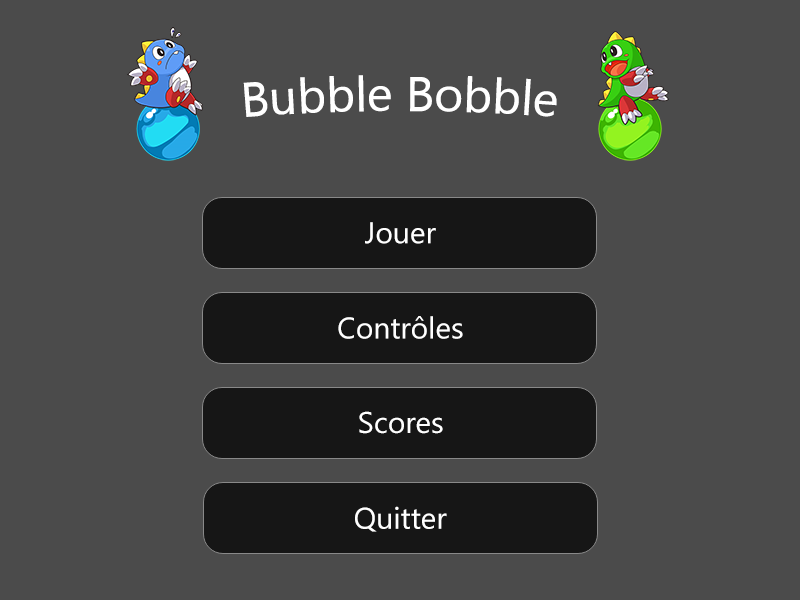
\includegraphics[width=400px]{Images/MainScreen.png}
		\caption{\'Ecran d'accueil}
		\label{fig:mainScreen}
	\end{center}
\end{figure}

\subsubsection{Contr\^oles}

Cet \'ecran (Figure~\ref{fig:loadingScreen}) sera affich\'e avant chaque partie afin de pr\'esenter au joueur les contr\^oles du jeu afin qu'il puisse facilement savoir comment jouer au jeu.

\begin{figure}[htbp]
	\begin{center}
		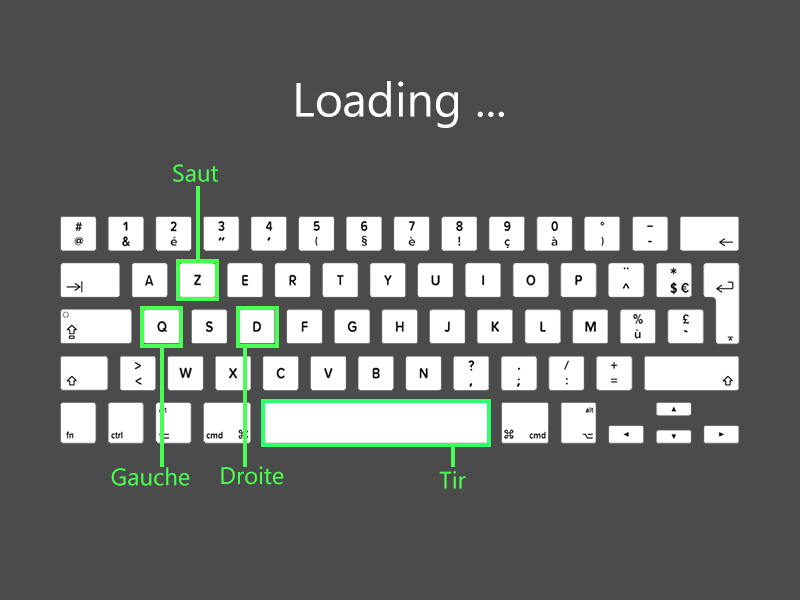
\includegraphics[width=400px]{Images/Loading.png}
		\caption{\'Ecran des contr\^oles affich\'es au chargement}
		\label{fig:loadingScreen}
	\end{center}
\end{figure}

\subsubsection{Jeu}

\'Ecran principal de l'application (Figure~\ref{fig:gameScreen}). Il pr\'esentera le niveau ainsi que certaines informations au joueur. Le score du joueur sera affich\'e en haut \`a gauche, le niveau en haut \`a droite et le nombre de vie, en bas \`a gauche.

\begin{figure}[htb]
	\begin{center}
		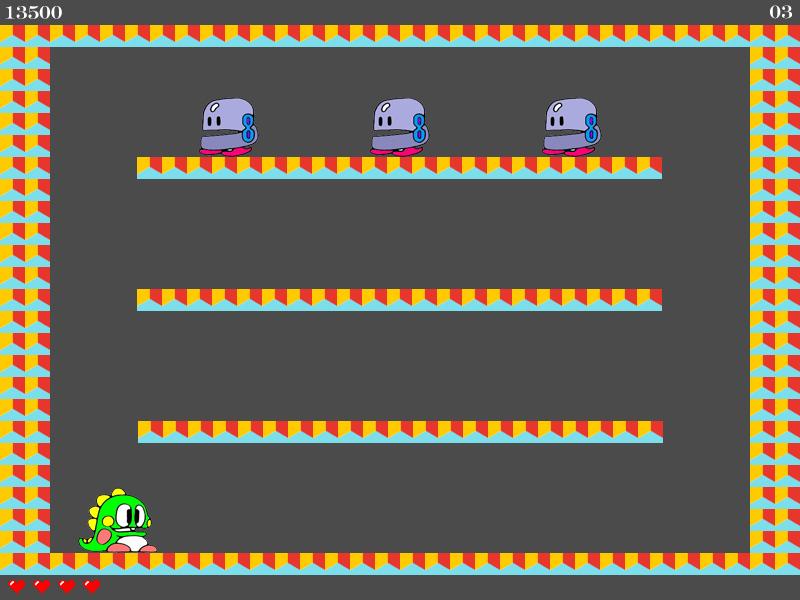
\includegraphics[width=400px]{Images/Game.png}
		\caption{\'Ecran de jeu}
		\label{fig:gameScreen}
	\end{center}
\end{figure}

\subsection{Fonctionnement du coeur du jeu}

Cette section d'\'ecrira les diff�rents \'el\'ements pour le fonctionnement du jeu. Comment le monde est repr\'esent\'e ou comment la d\'etection entre deux \'el\'ements du jeu sera d\'etect\'e.

\subsubsection{Repr\'esentation de la carte}

La carte sera divis\'e en une grille de 32 cellules de large sur 25 cellules de haut. Chaque cellule de cette grille sera un mur ou une zone vide. Ensuite, chaque bloc aura une taille de 25 pixels de large sur 22 pixels de haut.

\subsubsection{Repr\'esentation des personnages}

Les personnages du jeu, que \c ca soit pour le joueur ou pour les ennemis, seront repr\'esent\'es \`a l'aide d'une image qui sera positionn\'ee sur un axe x-y. Le personnage sera entour\'e d'une ``hitbox"~\cite{valve-hitbox}. La hitbox sera un rectangle qui entour le personnage (voir exemple figure~\ref{fig:hitbox}). Ce rectangle permettra de savoir quand deux \'el\'ements entre en collision. En effet, lorsque la position d'une ``hitbox" rencontre une autre ``hitbox", cela signifie que deux personnes se sont rencontr\'es.

\begin{figure}[htb]
	\begin{center}
		
\includegraphics[width=100px]{Images/Hitbox.png}
		\caption{La ``hitbox" est repr\'esent\'ee en rouge}
		\label{fig:hitbox}
	\end{center}
\end{figure}

Le m\^eme syst\`eme sera utilis\'e pour les bulles lanc\'ees par le joueur. M\^eme si les bulles sont repr\'esent\'es via une image ronde, la ``hitbox" de celles-ci seront aussi des rectangles afin de faciliter les calculs li\'es \`a la d\'etection de ``hit".

\subsection{Stuctures utilis\'ees}

\subsection{D\'ecoupage du code}

\section{Conclusion}

La principale difficult\'e de se projet va r\'esider dans le fait d'optimiser la gestion des hitbox afin que l'application se soit pas ralentie par la recherche de collision. En effet, \`a chaque tour de la boucle principale de GLUT, on va devoir v\'erifier si deux \'el\'ements sont entr\'es en collision, il faut donc optimiser au maximum cette gestion.

La deuxi\`eme difficult\'e sera l'utilisation de la biblioth\`eque GLUT. Celle-ci \'etant une bilioth\`eque ayant d\'ej\`a un certain nombre d'ann\'ee, il peut \^etre difficile de trouver certaines documentations ou alors les exemples pr\'esent\'es pour OpenGL utilisent de nouvelles biblioth\`eques.

\section{References}

\bibliographystyle{IEEEtran}
% Import the .bib file
\bibliography{rapport}

\end{document}